\section{Dataset Realization}
For the creation of our dataset, we devised a procedure that
allowed us to obtain a single file, in CSV format, where for
each timestamp, we have all the data for the entire system at
that exact moment. Below is the final structure of the dataset
and the algorithm for generating it.

%Per la realizzazione del nostro dataset abbiamo ideato 
%una procedura che ci ha permesso di ottenere un unico file,
%in formato csv, dove, per ogni time stamp abbiamo tutti i dati
%di tutto l'impianto in quell'esatto istante. Di seguito 
%la struttira finale del dataset e l'algoritmo per generarlo.


\begin{table}[H]
	\begin{center}
		\begin{tabular}[c]{l|l|l|l}
			\hline
			\multicolumn{1}{c|}{\textbf{timestamp}}              &
			\multicolumn{1}{c|}{\textbf{DEV.NAME$_1$\_FEAT$_1$}} &
			\multicolumn{1}{c|}{$\ldots$}                        &
			\multicolumn{1}{c}{\textbf{DEV.NAME$_n$\_FEAT$_n$}}                                   \\
			\hline

			01/10/2022 10:00                                     & $\ldots$ & $\ldots$ & $\ldots$ \\
			01/10/2022 10:05                                     & $\ldots$ & $\ldots$ & $\ldots$ \\
			01/10/2022 10:10                                     & $\ldots$ & $\ldots$ & $\ldots$ \\
			\hline
		\end{tabular}
	\end{center}
	\caption{Final dataset feature structure.}\label{tab:datasetform}
\end{table}

\begin{algorithm}[H]
	\caption{Dataset aggragation algorithm}\label{alg:dataset}
	\begin{algorithmic}
		\Require data\_folder
		\Ensure \texttt{data\_folder} exists
		\State dev\_types $\gets$ find all file types inside \texttt{data\_folder} (e.g. meter, inverter, $\ldots$)
		\State dev\_content $\gets$ a dictionary with \texttt{dev\_types} types as $keys$ and empty $values$

		\For {\textbf{each} key \textbf{in} dev\_conent.keys}
		\State files $\gets$ find all file matching type \texttt{key} inside \texttt{data\_folder}
		\State sort \texttt{files} by date (asc.)
		\State temp\_type\_aggregate $\gets$ and empty csv table
		\For {\textbf{each} file \textbf{in} files}
		\State append all \texttt{file} lines to \texttt{temp\_type\_aggregate} table
		\EndFor
		\State dev\_content[key] $\gets$ temp\_type\_aggregate
		\EndFor
		\State\Comment{At this time we have a dictionary mapping a file type with all its available data}
		\State
		\State dataset $\gets$ an empty csv table
		\For {\textbf{each} type, data \textbf{in} dev\_content} \Comment{\texttt{type} is $key$, \texttt{data} is $value$}
		\State rename all \texttt{data} $columns$ to \texttt{data.deviceID}\_\texttt{$column$.name}
		\State except for 'timestamp' $column$
		\State dataset $\gets$ merge \texttt{dataset} and \texttt{data} tables using 'timestamp' column
		\EndFor
		\State save \texttt{dataset} table to file
	\end{algorithmic}
\end{algorithm}

\begin{table}[H]
	\begin{center}
		\begin{tabular}[c]{l|l|l|l}
			\hline
			\multicolumn{1}{c|}{\textbf{timestamp}}      &
			\multicolumn{1}{c|}{\textbf{INV01\_PowerAC}} &
			\multicolumn{1}{c|}{\textbf{$\ldots$}}       &
			\multicolumn{1}{c}{\textbf{Cont\_TotalEnergy}}                                 \\
			\hline
			2022-02-02 00:05:00                          & NaN      & $\ldots$ & NaN       \\
			2022-02-02 00:10:00                          & NaN      & $\ldots$ & NaN       \\
			$\ldots$                                     & $\ldots$ & $\ldots$ & $\ldots$  \\
			2022-06-22 10:20:00                          & 175.66   & $\ldots$ & 8900941.5 \\
			2022-06-22 10:25:00                          & 178.29   & $\ldots$ & 8900995.5 \\
			2022-06-22 10:30:00                          & 180.82   & $\ldots$ & 8901036.0 \\
			$\ldots$                                     & $\ldots$ & $\ldots$ & $\ldots$  \\
			2023-06-16 18:00:00                          & NaN      & $\ldots$ & NaN       \\
			2023-06-16 18:05:00                          & NaN      & $\ldots$ & NaN       \\
		\end{tabular}
	\end{center}
	\caption{Some data from dataset after running Algorithm \ref{alg:dataset}}\label{tab:datasetfinalvalues}
\end{table}

\subsection{Timestamp cyclical encoding}
To enable the models to learn the alternation of minutes, days,
and months as effectively as possible during the training phase,
we applied a procedure to transform each individual timestamp into
a pair of sine and cosine values, thus performing a cyclic
encoding of various seasonalities.

%Per permettere ai modelli, durante la fase di allenamento, di apprendere
%al meglio possibile l'alternarsi dei minuti, giorni e mesi abbiamo
%applicato una procedura per trasfrormare ogni signolo timestamp
%in una coppia di valori seno-coseno effettuando così un 
%encoding ciclico delle varie stagionalità.


\begin{algorithm}[H]
	\caption{Cyclical Encoding Algorithm}\label{alg:cyclicencoding}
	\begin{algorithmic}
		\Require dataset table
		\Ensure \texttt{dataset} \textbf{is not} empty
		\State dataset['minute\_sin'] $\gets \sin(2 \pi (\frac{\text{\texttt{dataset.timestamp.minute}}}{60}))$
		\State dataset['minute\_cos'] $\gets \cos(2 \pi (\frac{\text{\texttt{dataset.timestamp.minute}}}{60}))$


		\State dataset['hour\_sin'] $\gets \sin(2 \pi (\frac{\text{\texttt{dataset.timestamp.hour}}}{24}))$
		\State dataset['hour\_cos'] $\gets \cos(2 \pi (\frac{\text{\texttt{dataset.timestamp.hour}}}{24}))$


		\State dataset['day\_sin'] $\gets \sin(2 \pi (\frac{\text{\texttt{dataset.timestamp.day}}}{31}))$
		\State dataset['day\_cos'] $\gets \cos(2 \pi (\frac{\text{\texttt{dataset.timestamp.day}}}{31}))$

		\State dataset['month\_sin'] $\gets \sin(2 \pi (\frac{\text{\texttt{dataset.timestamp.month}}}{12}))$
		\State dataset['month\_cos'] $\gets \cos(2 \pi (\frac{\text{\texttt{dataset.timestamp.month}}}{12}))$
	\end{algorithmic}
\end{algorithm}

\begin{figure}[H]
	\centering
	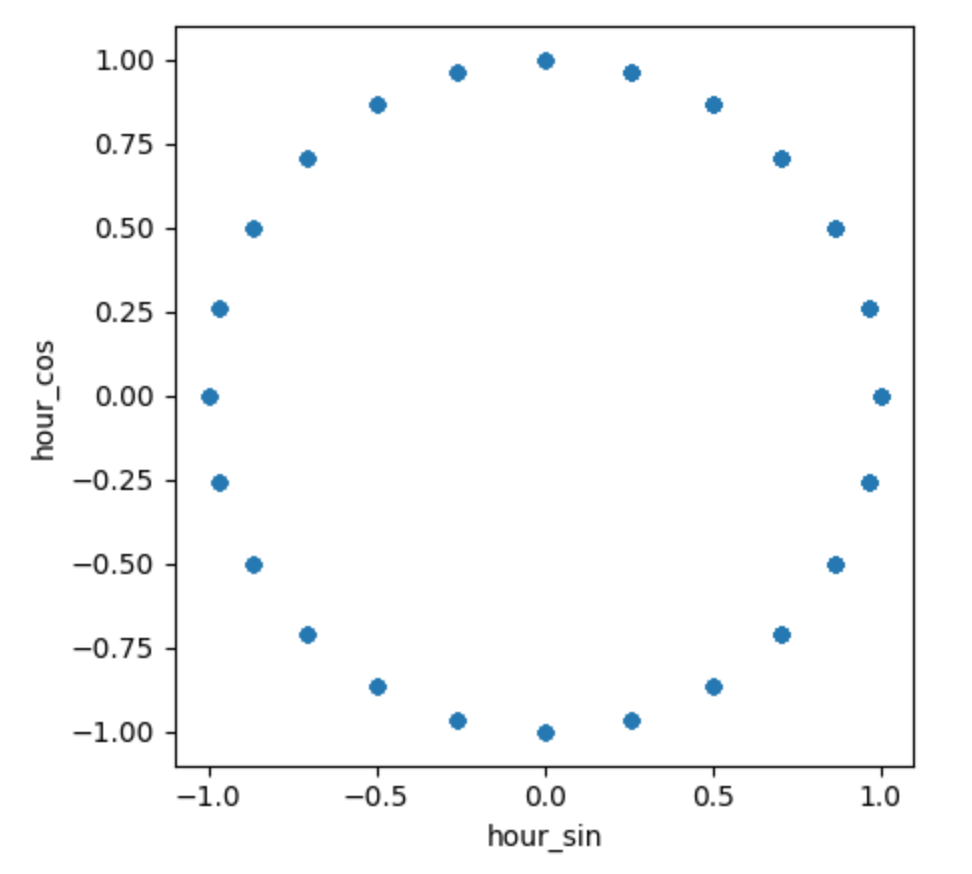
\includegraphics[width=0.7\linewidth, keepaspectratio]{chapters/2_data_preprocessing/imgs/hoursincosplot.png}
	\caption{Hour cyclical encoding plot.}
	\label{fig:encodingplot}
\end{figure}

\subsection{Dealing with Holes}

\begin{figure}[H]
	\centering
	\begin{subfigure}[t]{0.48\textwidth}
		\centering
		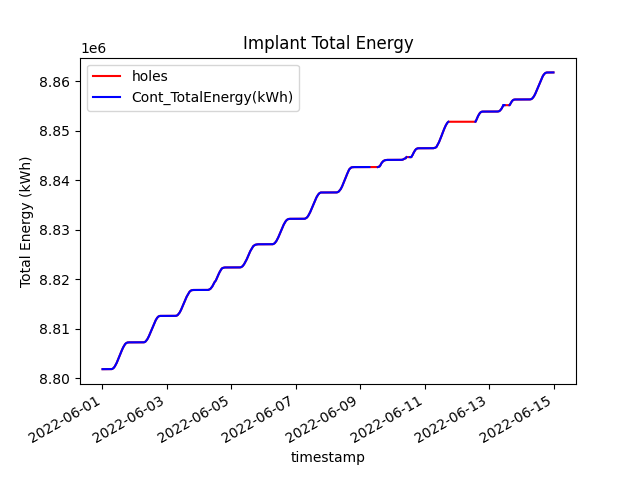
\includegraphics[width=\textwidth, keepaspectratio]{chapters/2_data_preprocessing/imgs/totenergybuco1.png}
	\end{subfigure}
	\hspace{0.1cm}
	\begin{subfigure}[t]{0.48\textwidth}
		\centering
		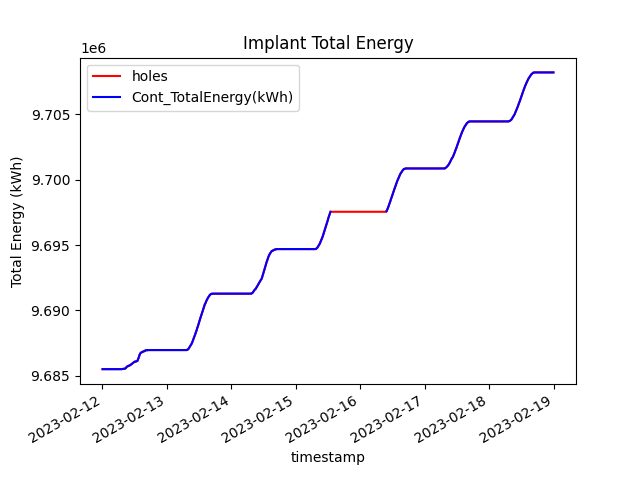
\includegraphics[width=\textwidth, keepaspectratio]{chapters/2_data_preprocessing/imgs/totenergybuco2.png}
	\end{subfigure}\\

	\begin{subfigure}[t]{0.48\textwidth}
		\centering
		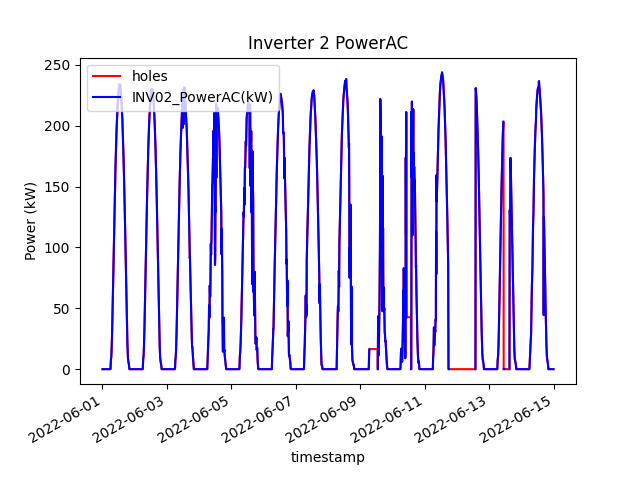
\includegraphics[width=\textwidth, keepaspectratio]{chapters/2_data_preprocessing/imgs/inv02powerbuco1.png}
	\end{subfigure}
	\hspace{0.1cm}
	\begin{subfigure}[t]{0.48\textwidth}
		\centering
		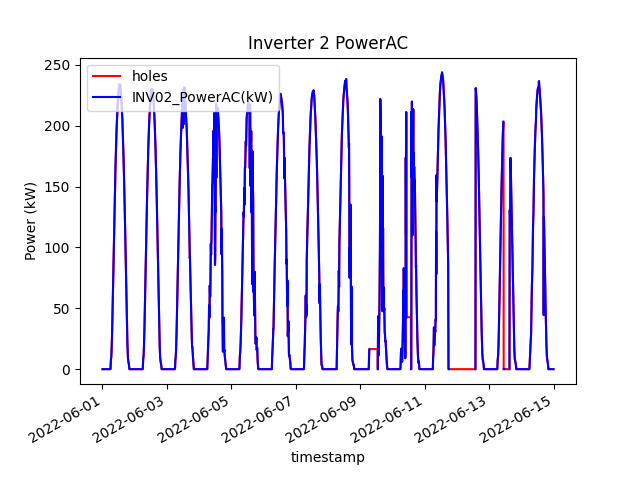
\includegraphics[width=\textwidth, keepaspectratio]{chapters/2_data_preprocessing/imgs/inv02powerbuco1.png}
	\end{subfigure}
	\caption{Some dataset \textquote{holes}. The charts at the top refer to the Implant's Total Energy, while those at the bottom refer to the Inverter 2's Power. The charts on the left range from 01-06-2022 to 15-06-2022, while those on the right range from 12-02-2023 to 19-02-2023.}
	\label{fig:graficibuchi}
\end{figure}

As we can see from Figure \ref{fig:graficibuchi}, there are certain
periods within the dataset (highlighted in red) where data is missing,
which we refer to as \textquote{holes}. Leaving these gaps in the
dataset causes problems during model training
(hindering the correct calculation of the loss function), and therefore,
they need to be removed. One possible approach for holes removal
is to perform a \textit{fill} operation: filling the gap with the
first available non-null value. This tactic may be considered
acceptable only if the time span involves just a few timestamps.
However, if we are talking about several hours or even days, it
significantly distorts the overall production and instantaneous
power trends, resulting, especially in very unfortunate cases, with extremely abnormal production curves.

The solution we have adopted to address this problem is the removal of
the entire day when a hole occurs. For example, if we have a data
gap from 12-02-2023 23:00 to 13-02-2023 10:40, the days
12-02-2023 and 13-02-2023 will be completely removed. With this
method, we lose some data, but as we will see later, the number of
gaps is not extremely high, and this data loss is not
debilitating. The following algorithm summarizes what has
just been described.

%Come possiamo vedere dalla Figura \ref{fig:graficibuchi}, all'interno del dataset sono presenti alcuni periodi (evidenziati in rosso) di assenza dati che è ciò che chiamiamo \textquote{buco}.
%Lasciare questi buchi causa problemi durante l'allenamento dei modelli (impediscono il corretto calcolo della loss function) e per questo
%vanno rimossi. Un possibile approccio per la loro rimozione è effettuare
%un'operazione di \textquote{fill}: riempio il buco con il primo valore non nullo disponibile.
%Questa tattica può essere ritenuta accettabile solo se il lasso di tempo coinvolge solo qualche timestamp, se invece parliamo di
%qualche ora o addirittura giorni questo va ad alterare notevolmente
%l'andamento della produzione totale e della potenza istantanea, risultando in casi molto sfortunati, ad avere curve di produzione estremamente anomale.
%
%La soluzione che abbiamo adottato per risolvere questo problema è
%l'eliminazione di tutto il giorno in cui si presenta il buco.
%Per fare un esempio pratico, se abbiamo un buco di dati che va dal
%12-02-2023 23:00 al 13-02-2023 10:40, verranno completamente eliminati
%i giorni 12-02-2023 e 13-02-2023. Con questo metodo andiamo a perdere 
%alcuni dati, ma come vedremo poi, il numero dei buchi non è estremamente
%elevato e la perdita di questi dati non risulta invalidante. Il seguente algoritmo riassume quanto appena detto.
%
\noindent\begin{minipage}[t]{0.55\linewidth}
	\begin{algorithm}[H]
		\caption{Holes Removal Algorithm.}\label{alg:holes}
		\begin{algorithmic}
			\Require dataset table
			\Ensure \texttt{dataset} \textbf{is not} empty

			\State holes $\gets$ find all timestamp from \texttt{dataset} table, where there are some \texttt{Nan}s inside the columns
			\For{\textbf{each} row \textbf{in} \texttt{dataset.rows}}
			\If {row.timestamp \textbf{is in} \texttt{holes}}
			\State drop \texttt{row} from \texttt{dataset} table
			\EndIf
			\EndFor
		\end{algorithmic}
	\end{algorithm}

\end{minipage}%
\hfill%
\begin{minipage}[t]{0.30\linewidth}
	\begin{table}[H]
		\centering
		\begin{tabular}[c]{l}
			\multicolumn{1}{c}{\textbf{Timestamp}} \\
			\hline
			2022-06-09                             \\
			2022-06-10                             \\
			2022-06-11                             \\
			2022-06-12                             \\
			2022-06-13                             \\
			2022-06-28                             \\
			2022-06-29                             \\
			2022-06-30                             \\
			2022-08-26                             \\
			2022-09-23                             \\
			2022-10-06                             \\
			2023-02-03                             \\
			2023-02-15                             \\
			2023-02-16                             \\
			2023-03-26                             \\
		\end{tabular}
		\caption{Timestamps deleted after running the Algorithm \ref{alg:holes}}
	\end{table}
\end{minipage}


\subsection{Historical weather}
